\section{Label Consistent K-SVD}
\cite{6516503} proposed a supervised learning algorithm to learn a compact and discriminative dictionary for sparse coding. They add a new label consistency constraint ( ``discriminative sparse-code error") and combining reconstruction error and classification error to form a unified objective function that can be solved with the K-SVD algorithm.
%\subsection{Dictionary Learning for classification}
%A good classifier $f(x)$ can be obtained by determining its model parameters $W \in R^{m \times K} $ satisfying:
%\begin{center}
% $W = \underset{W}{\argmin} \underset{i}{\sum}\mathcal{L}\{h_i,f(x_i,W)\} + \lambda_1 \|W\|^2_F$
%\end{center}
%where: $m$ is the number of classes, $\mathcal{L}$ is the classification loss function (typically logistic loss function, suqare hinge loss, simple quadratic loss function), $h_i$ the label of $y_i$ and $\lambda_1$ a regularization parameters (which prevents overfitting).\\
%The objective function for learning $D$ and $W$ jointly can be :
%\begin{center}
 %$<D,W,\alpha> = \underset{D,W,\alpha}{\argmin} \|X -D\alpha\|^2_2 + \underset{i}{\sum}\mathcal{L}\{h_i,f(\alpha_i,W)\} + \lambda_1 \|W\|^2_F$  s.t.  $\forall i, \|\alpha_i\|_0 \leq T$ 
%\end{center}

%The sparse code $\alpha_i$ can be used as a feature descriptor of input signal $x_i$, then the risk minimization formulation can be written as:
%\begin{center}
 %$<D,W> = \underset{D,W}{\argmin}\underset{i}{\sum}\mathcal{L}\{h_i,f(\alpha^*(x_i,D),W)\} + \frac{\nu_1}{2}\|W\|^2_F$
%\end{center}
%Here D is not explicitly defined in the function but implicitlu in the sparse coding step ($\alpha^*(x_i,D)$ )

\subsection{Idea}
In a supervised setting, during the training phase, all the information about an input signal is given, including its label. The idea is to use this information to learn a discriminative dictionary. To do this, \cite{6516503} add a new consistency regularization term, a classification error and label consistency regularization term into the objective function:
\begin{center}
 $<D,\gamma> = \underset{D,\gamma}{\argmin} \|X - D\gamma\|^2_2 + \lambda \|\gamma\|_0 +\underset{Label\ consistent\ term}{\underbrace{\mu \|Q -AX\|_2^2 }} + \underset{Consistency\ term}{\underbrace{\beta\|H-WH\|_2^2}}$
\end{center}
%They refer to this two problem as LC-KSVD1 and LC-KSVD2 respectivly.
Where Q is the discriminative sparse codes of input signals X for classification, A is a linear transformation matrix, W is the classifier parameters and H is the labels corresponding to the input signal X.\\
This optimization function is called LC-KSVD2. But there is a variant of this method, called LC-KSVD1 which is the same function without the consistency term.\\
In our setting, we will use LC-KSVD1 because we do not want to train a classifier at this stage.
\subsection{LC-KSVD1}
Therefore, the objective function for dictionary learning is  defined as:
\begin{center}
 $<D,A,\gamma> = \underset{D,A,\gamma}{\argmin} \| X - D\gamma \|^2_2 + \mu \|Q -A\gamma\|^2_2 + \lambda\|\gamma\|_0$
\end{center}

Where $\mu$ controls the contribution between reconstruction and label consistency regularization. $Q = [q_1,...,q_N] \in \R^{K \times N}$.\\
Q is a discriminative sparse code corresponding to an input signal and the dictionary atoms, the nonzero values occur when $signal_i$ and $atom_i$ share the same label (figure \ref{fig:Q}).\\
Q is chosen by the user, in our setting we have chosen to match the same number of atoms for each class. It is then possible to have "empty" atoms that are not discriminative (white color's atom in figure \ref{fig:Q}).
\begin{figure}[h]
 \centering
 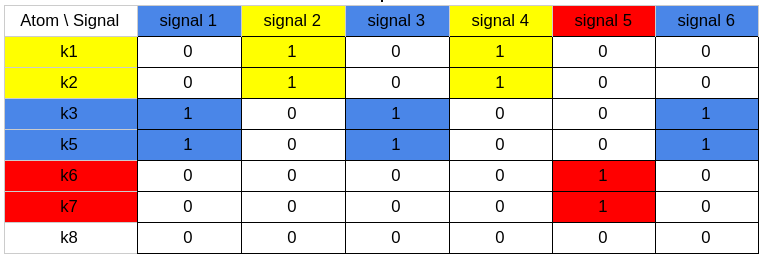
\includegraphics[scale=0.7]{LCKSVDTable.png}
 % Q_explications.png: 487x177 px, 96dpi, 12.88x4.68 cm, bb=0 0 365 133
 \caption{Example of Q, each color corresponding to a class (white color is the lack of classes). Signal 1,3 and 6 are from class 1; signal 2 and 5 from class 2 and signal 5 from class 3}
  \label{fig:Q}

\end{figure}
To use K-SVD algorithm it is necessary to  rewrite the previous equation:
\begin{center}
$ <D,A,\gamma> = \underset{D,A,\gamma}{\argmin} \| \begin{pmatrix} 
X  \\
\sqrt{\mu}Q
\end{pmatrix} -  \begin{pmatrix} 
D  \\
\sqrt{\mu}A
\end{pmatrix}\gamma \|^2_2\lambda \|\gamma\|_0$
\end{center}
We define $X_{new}  =  \begin{pmatrix} 
X  \\
\sqrt{\mu}Q
\end{pmatrix}$ and $D_{new} =  \begin{pmatrix} 
D  \\
\sqrt{\mu}A
\end{pmatrix}$. \\ \hspace{0.5cm}
It's important to note that the $D_{new}$ matrix is $L_2$ normalized. Now, it is possible to solve the minimization problem using the K-SVD algorithm:
\begin{center}
 $<D,A,\gamma> = \underset{D,A,\gamma}{\argmin} \| X_{new} - D_{new}\gamma \|^2_2 + \lambda \|\gamma\|_0$
\end{center}
However, it is impossible to use directly D and A  after employing the K-SVD algorithm. It is because D and A are $L_2$ normalized due to $D_{new}$. The desired $\hat{D}$ and $\hat{A}$ can be computed as follows:\vspace{0.5cm}\begin{center}
$\hat{D} = (
\frac{d_1}{\|d1\|_2}  ...  \frac{d_K}{\|d_K\|_2} 
)$   and $\hat{A} =
(\frac{a_1}{\|d_1\|_2}  ...  \frac{a_K}{\|d_K\|_2} 
)$
\end{center}
Label-Consistent K-SVD algorithm is given as follow:
\begin{algorithm}
 \caption{Label Consistent K-SVD 1 (LC-KSVD1)}
 \begin{algorithmic}
  \REQUIRE $X, Q, \lambda_1$
  \STATE $D_0$ = KSVD($X, \lambda_1$)
  \STATE $A_0 = Q  X^{\intercal} (X  X^{\intercal} + \lambda_2  I)^{-1}$
  \STATE $\gamma_0$ = OMP($D_0, X, lambda_1$)
  \STATE $X_{new}  =  \begin{pmatrix} 
    X  \\
    \sqrt{\mu}Q
    \end{pmatrix}$
  \STATE $D_{new} =  \begin{pmatrix} 
    D  \\
    \sqrt{\mu}A
    \end{pmatrix}$
  \STATE $ D = $ KSVD($D_{new}, X_{new}, \lambda_1)$
  \STATE $\hat{D} = (
\frac{d_1}{\|d1\|_2}  ...  \frac{d_K}{\|d_K\|_2} 
)$
\STATE $\hat{A} =
(\frac{a_1}{\|d_1\|_2}  ...  \frac{a_K}{\|d_K\|_2} 
)$
\RETURN $\hat{D}, \hat{A}$
 \end{algorithmic}

\end{algorithm}

%\vspace{0.5cm}
%\begin{lstlisting}[language=Python,frame=single]
%Input: X, Q, lambda1, K
%Output: D, A
%===========================================================================
%D_0 = K-SVD(X,lambda1)
%A_0 = Q * tranpose(X) * inv(X*tranpose(X) + lamba2 * Id)
%h_0 = omp(Dnew,Xnew,lambda1)

%Initialize Xnew and Dnew
%D = K-SVD(Dnew,Xnew,lambda1)

%Extract D, A
%return D, A
%\end{lstlisting}
%\vspace{0.5cm}
%With $A_0 = Q X^T (XX^T + \lambda_2 I)^{-1}$
%\vspace{0.5cm}\\
%In our case we don't want to train the classifier, we only want to find new features. This is why we only apply LC-KSVD1.\\
%You can find my Python code of  LC-KSVD1 on MNIST in my Github repository: \texttt{LC-KSVD.py}
